\subsection{New Product Process}
\begin{frame}
  \frametitle{Development Challenges}
  \framesubtitle{Regulatory Barrier}
  \begin{figure}
    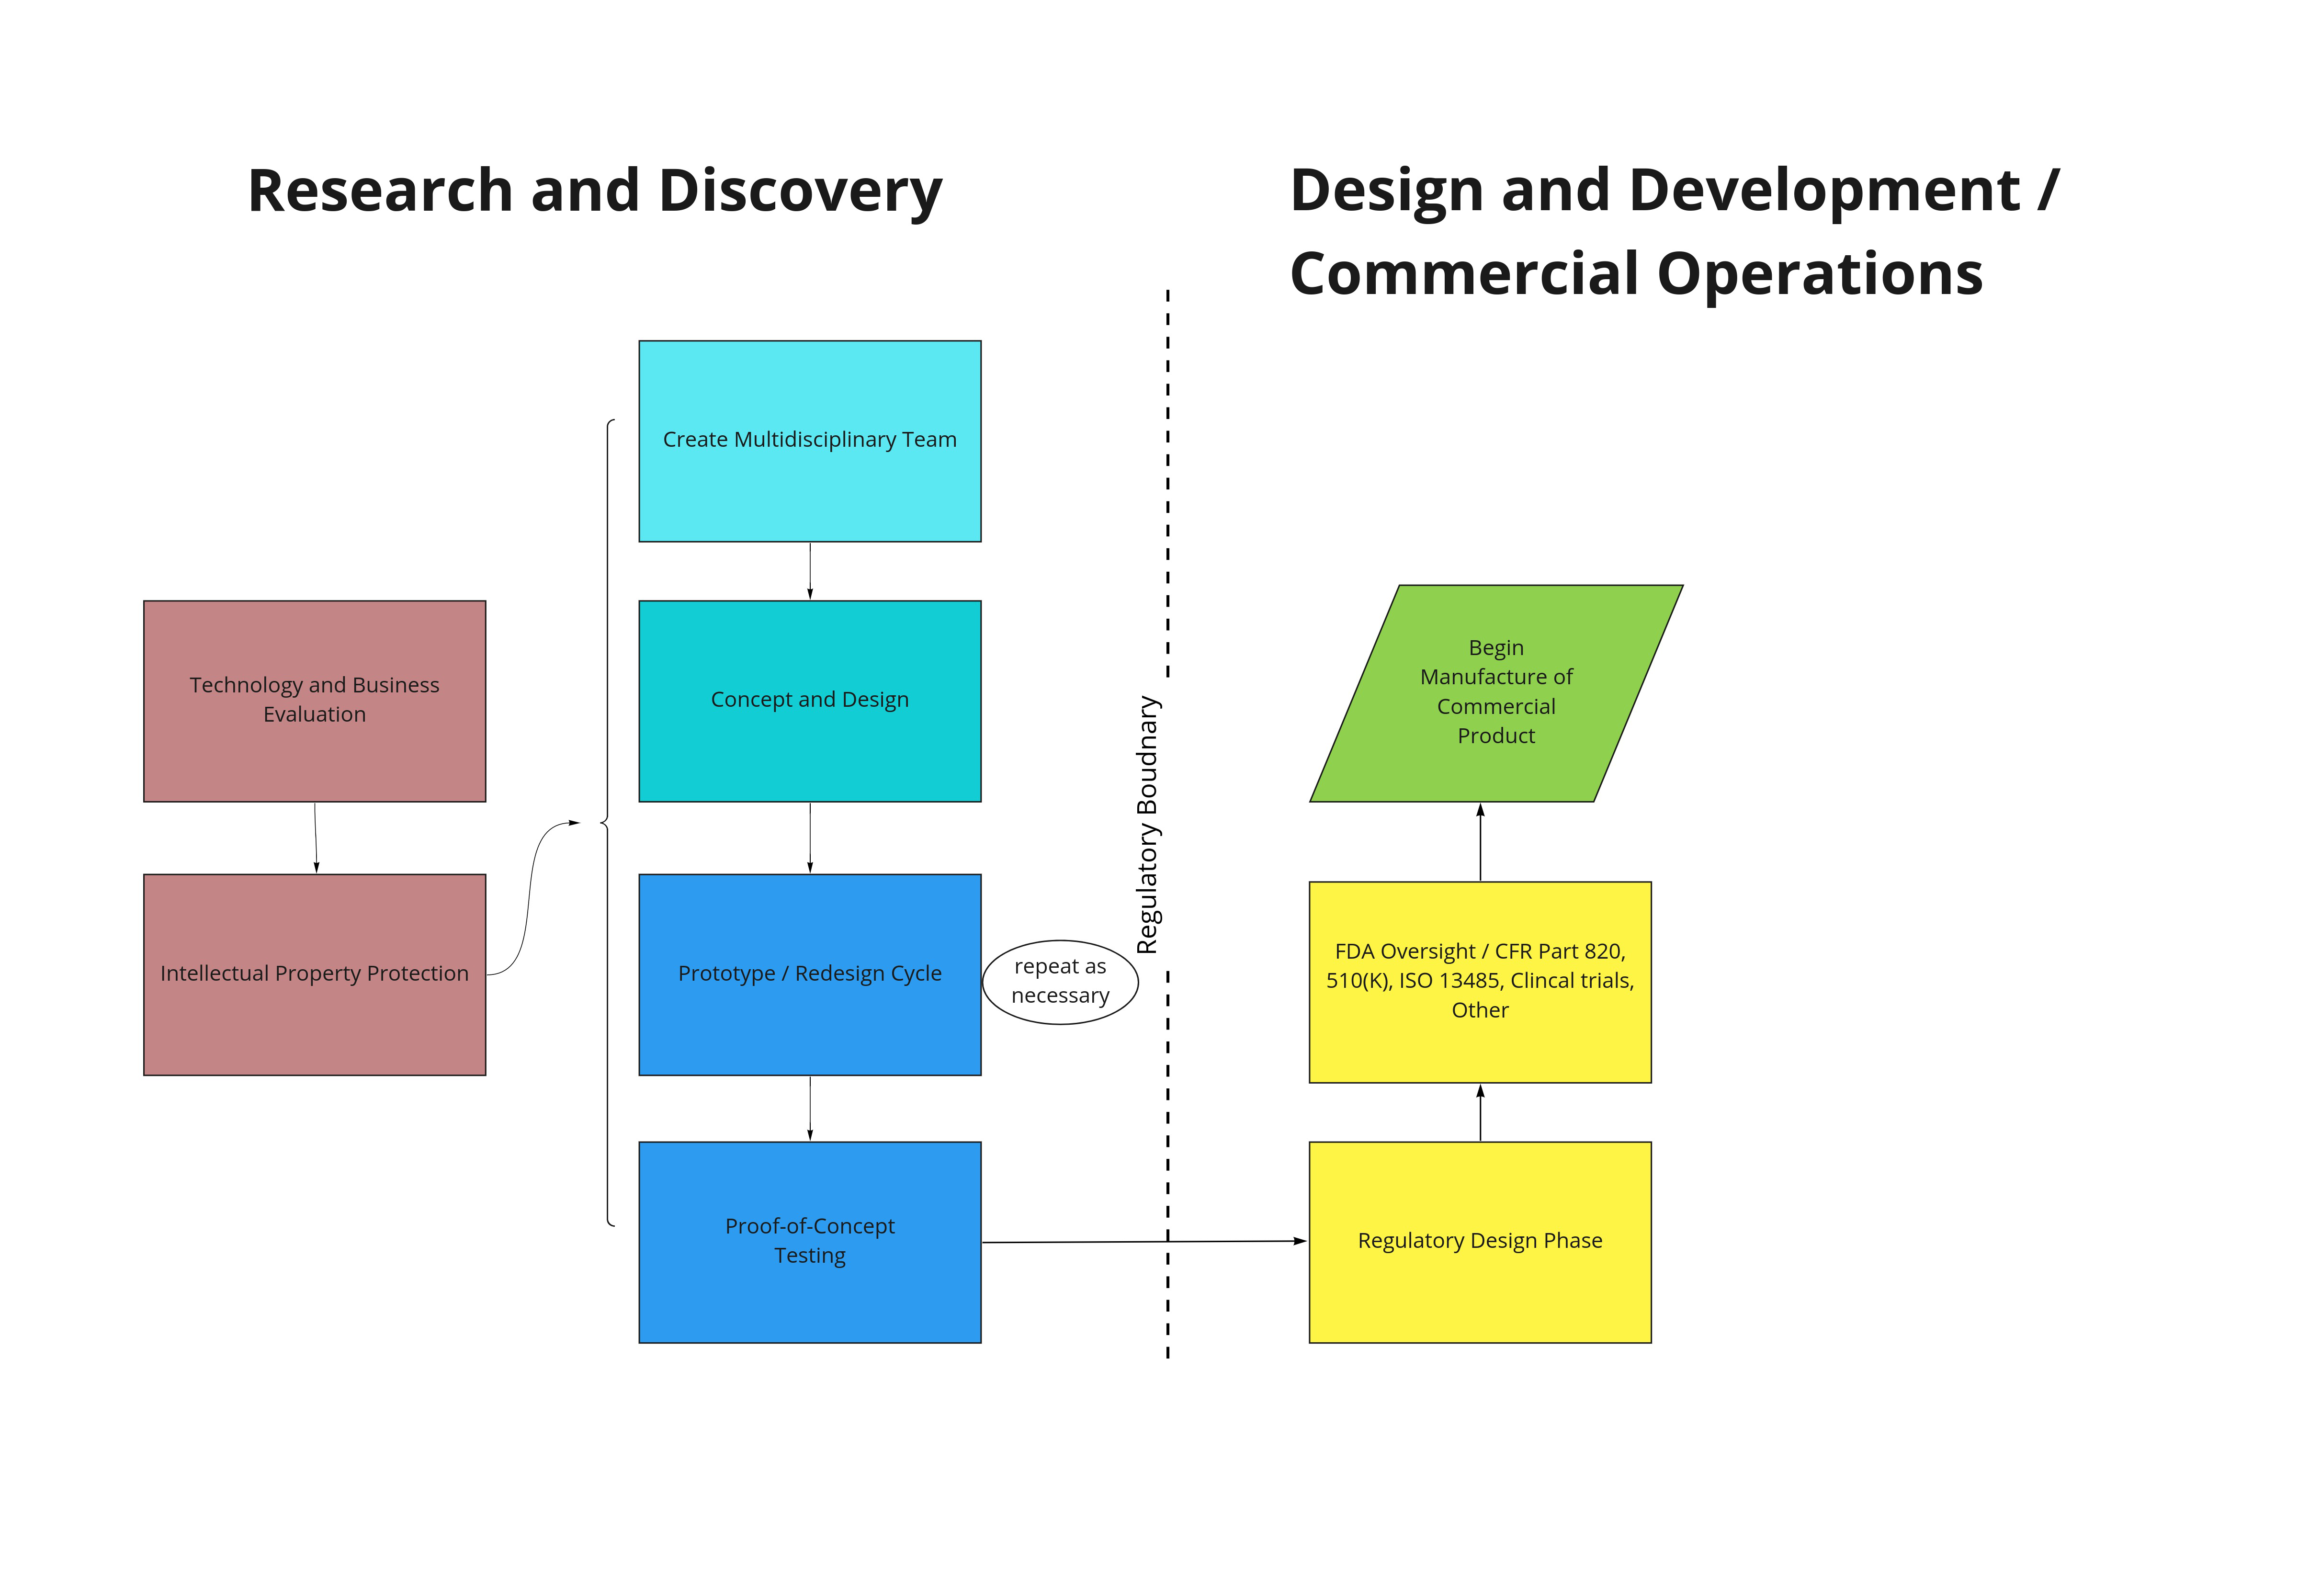
\includegraphics[width=\textwidth]{img/medical}
    \caption{Image from \textcite{dasUseManufacturingTechnologiesan2010}}
\end{figure}

\note[item]{\scriptsize{Two critical aspects of to note about the specific challenges of operations management in the medical device manufacturing production process are the interactions of an enourmous number of regulations that overlap throughout the product development and production process along with the reality that once in the clinical trial phase, partial commercial production needs to be already established. It is not the case that clinical approvals are conducted on prototypes. Rather, approvals are granted based on the commercial production process. This means that operational production facilities need to be established at a small scale and maintained throughout the clinical approval period. As was noted this period averages well over 200 days for Class III devices. This creates a non-trivial burden for establishing a commercial product, as the production facilities need to scale with demand, but demand can not be established until the regulatory burdens have been met. [Image derrived from \textcite{dasUseManufacturingTechnologiesan2010}]}}

\end{frame}
